\documentclass{sigchi}

% Use this section to set the ACM copyright statement (e.g. for
% preprints).  Consult the conference website for the camera-ready
% copyright statement.

% Copyright
\CopyrightYear{2016}
%\setcopyright{acmcopyright}
\setcopyright{acmlicensed}
%\setcopyright{rightsretained}
%\setcopyright{usgov}
%\setcopyright{usgovmixed}
%\setcopyright{cagov}
%\setcopyright{cagovmixed}
% DOI
\doi{http://dx.doi.org/10.475/123_4}
% ISBN
\isbn{123-4567-24-567/08/06}
%Conference
\conferenceinfo{CHI'16,}{May 07--12, 2016, San Jose, CA, USA}
%Price
\acmPrice{\$15.00}

% Use this command to override the default ACM copyright statement
% (e.g. for preprints).  Consult the conference website for the
% camera-ready copyright statement.

%% HOW TO OVERRIDE THE DEFAULT COPYRIGHT STRIP --
%% Please note you need to make sure the copy for your specific
%% license is used here!
% \toappear{
% Permission to make digital or hard copies of all or part of this work
% for personal or classroom use is granted without fee provided that
% copies are not made or distributed for profit or commercial advantage
% and that copies bear this notice and the full citation on the first
% page. Copyrights for components of this work owned by others than ACM
% must be honored. Abstracting with credit is permitted. To copy
% otherwise, or republish, to post on servers or to redistribute to
% lists, requires prior specific permission and/or a fee. Request
% permissions from \href{mailto:Permissions@acm.org}{Permissions@acm.org}. \\
% \emph{CHI '16},  May 07--12, 2016, San Jose, CA, USA \\
% ACM xxx-x-xxxx-xxxx-x/xx/xx\ldots \$15.00 \\
% DOI: \url{http://dx.doi.org/xx.xxxx/xxxxxxx.xxxxxxx}
% }

% Arabic page numbers for submission.  Remove this line to eliminate
% page numbers for the camera ready copy
% \pagenumbering{arabic}

% Load basic packages
\usepackage{balance}       % to better equalize the last page
\usepackage{graphics}      % for EPS, load graphicx instead 
\usepackage[T1]{fontenc}   % for umlauts and other diaeresis
\usepackage{txfonts}
\usepackage{mathptmx}
\usepackage[pdflang={en-US},pdftex]{hyperref}
\usepackage{color}
\usepackage{booktabs}
\usepackage{textcomp}

% Some optional stuff you might like/need.
\usepackage{microtype}        % Improved Tracking and Kerning
% \usepackage[all]{hypcap}    % Fixes bug in hyperref caption linking
\usepackage{ccicons}          % Cite your images correctly!
% \usepackage[utf8]{inputenc} % for a UTF8 editor only

% If you want to use todo notes, marginpars etc. during creation of
% your draft document, you have to enable the "chi_draft" option for
% the document class. To do this, change the very first line to:
% "\documentclass[chi_draft]{sigchi}". You can then place todo notes
% by using the "\todo{...}"  command. Make sure to disable the draft
% option again before submitting your final document.
\usepackage{todonotes}
\usepackage{algorithm}
\usepackage{algpseudocode}
\usepackage{floating}

\let\oldReturn\Return
\renewcommand{\Return}{\State\oldReturn}
% Paper metadata (use plain text, for PDF inclusion and later
% re-using, if desired).  Use \emtpyauthor when submitting for review
% so you remain anonymous.
\def\plaintitle{A Vision-based Road Crossing Assistant System Empowered by Deep Learning}
\def\plainauthor{First Author, Second Author, Third Author,
  Fourth Author, Fifth Author, Sixth Author}
\def\emptyauthor{}
\def\plainkeywords{Computer Vision; Detection; Tracking}
\def\plaingeneralterms{Documentation, Standardization}
\newcommand{\para}[1]{\smallskip\noindent\textbf{#1}}

% llt: Define a global style for URLs, rather that the default one
\makeatletter
\def\url@leostyle{%
  \@ifundefined{selectfont}{
    \def\UrlFont{\sf}
  }{
    \def\UrlFont{\small\bf\ttfamily}
  }}
\makeatother
\urlstyle{leo}

% To make various LaTeX processors do the right thing with page size.
\def\pprw{8.5in}
\def\pprh{11in}
\special{papersize=\pprw,\pprh}
\setlength{\paperwidth}{\pprw}
\setlength{\paperheight}{\pprh}
\setlength{\pdfpagewidth}{\pprw}
\setlength{\pdfpageheight}{\pprh}

% Make sure hyperref comes last of your loaded packages, to give it a
% fighting chance of not being over-written, since its job is to
% redefine many LaTeX commands.
\definecolor{linkColor}{RGB}{6,125,233}
\hypersetup{%
  pdftitle={\plaintitle},
% Use \plainauthor for final version.
%  pdfauthor={\plainauthor},
  pdfauthor={\emptyauthor},
  pdfkeywords={\plainkeywords},
  pdfdisplaydoctitle=true, % For Accessibility
  bookmarksnumbered,
  pdfstartview={FitH},
  colorlinks,
  citecolor=black,
  filecolor=black,
  linkcolor=black,
  urlcolor=linkColor,
  breaklinks=true,
  hypertexnames=false
}

% create a shortcut to typeset table headings
% \newcommand\tabhead[1]{\small\textbf{#1}}

% End of preamble. Here it comes the document.
\begin{document}

\title{\plaintitle}

\numberofauthors{3}
\author{%
  \alignauthor{Leave Authors Anonymous\\
    \affaddr{for Submission}\\
    \affaddr{City, Country}\\
    \email{e-mail address}}\\
  \alignauthor{Leave Authors Anonymous\\
    \affaddr{for Submission}\\
    \affaddr{City, Country}\\
    \email{e-mail address}}\\
  \alignauthor{Leave Authors Anonymous\\
    \affaddr{for Submission}\\
    \affaddr{City, Country}\\
    \email{e-mail address}}\\
}

%\numberofauthors{4}
%\author{%
%  \alignauthor{Han Shen\\
%%  \affaddr{Institute for Interdisciplinary Information Sciences,}
%  \affaddr{Institute for Interdisciplinary Information Sciences, }
%    \affaddr{Tsinghua University, China}\\
%    \email{thushenhan@gmail.com}}\\
%  \alignauthor{Changcheng Tang\\
%    \affaddr{Institute of Microelectronics,}\\
%    \affaddr{Tsinghua University, China}\\
%    \email{tangcc1127@gmail.com}}\\
%  \alignauthor{Tianyi Lu\\
%    \affaddr{Institute of Microelectronics,}\\
%    \affaddr{Tsinghua University, China}\\
%    \email{thutianyi@outlook.com}}\\
%  \alignauthor{Binren Tian\\
%    \affaddr{Institute of Microelectronics,}\\
%    \affaddr{Tsinghua University, China}\\
%    \email{tian.br@foxmai.com}}\\
%}

\maketitle


\begin{abstract}
To ensure the safety of people with disabilities in public traffic environment has always been a formidable problem that plagues the community and the society. At the road intersections of traffic, how to guide visually impaired pedestrians to cross the roads independently has been a tough task. There is still an evident lack of relevant research works on this task. Nowadays, deep learning algorithms have achieved equivalent or even beyond human-level capability, especially in computer vision-based task. The fast-developing deep learning algorithms give us a chance to solve the task. In this paper, we proposed a vision-based auxiliary system that combines detection and tracking of zebra-crossing,  traffic lights and obstacles to help visually impaired pedestrians deal with complex urban road scenes when crossing the road intersections. Our application uses state-of-the-art deep learning algorithms together with efficient computer vision algorithms, which have been proven to be successful in a variety of usage scenarios.
\end{abstract}

\category{H.5.2.}{Information Interfaces and Presentation
	(e.g. HCI)}{User Interfaces} \category{}{}{}

\keywords{\plainkeywords}
\include{data/intro}
\include{data/related}
\section{Method}
\subsection{Problem Formulation}
The main difficulties for the blind people to cross the street include: 1) to find the direction to go; 2) to recognize the  traffic lights; 3) to distinguish and avoid obstacles through the road. In response to these problems, we have given corresponding solutions. The system is dedicated to be deployed in the form of smart glasses.

\para{Direction to go.} Modern smart phones already include sophisticated maps and navigation solutions. In order to guide the blind correctly, we ensure that the GPS of the smart glasses always points to the front of the blind person. Therefore, regardless of how the blind walks to the intersection, the path plan generated by the navigation app enables the blind person to roughly know the direction of the road he wants to cross.

\para{Recognition of traffic lights.} It is necessary to be aware of the traffic light status before crossing the road. Generally, the solution to the task is broken down into two parts: firstly to detect the position of the traffic light in the image; secondly to identify the light color in corresponding areas. Recently, to propel the development of automated driving, researchers have annotated an amount of datasets, including traffic signs, traffic lights, vehicles and pedestrians on road. Therefore, it's feasible to use a learning-based detection algorithm to detect the traffic lights. 

Inevitably, an image captured by an RGB camera may conclude multiple traffic lights. The problem of distinguishing the correct pedestrian light is not within the consideration of automated driving, but is indeed significant in our application. Unfortunately, the standard for the traffic lights in different countries is not unified. For instance, China uses the human figures to represent pedestrian lights, and the arrow figures to indicate left turn or right turn; While in the USA, both pedestrian lights and car lights are all indicated by red or green circular figures, which makes it difficult to directly differentiate the pedestrian light from shape. Nevertheless, we assume that there are zebra crossings  on city roads, so the traffic lights on the opposite side of the zebra crossing should be pedestrian lights. Thus, by detecting zebra lines on road, we use this intuition in our algorithms to identify pedestrian and non-pedestrian lights.

\para{Obstacle avoidance.} Even if green lights turns on, it doesn't mean that the blind can cross the road right away. There are always pedestrians from same or opposite sides walking back and forth; and it is possible that some vehicles are also making the left/right turn simultaneously, since that in certain countries, the left or right turn for the motor vehicles are not ruled by the traffic light; More commonly, non-motorized vehicles are also running on the non-motorized lanes on both sides. If not getting notified of how to avoid these obstacles in time, blind people will be in risk to walk through. Our solution is to first use the detection algorithm to obtain the position of obstacles in view, and secondly to obtain the distance between each obstacle and the blind by monocular or binocular depth estimation algorithms. Moreover, if we can predict the motion of the obstacle in future, we will be able to better decide whether to stop or keep forwarding, so we also track the route of the obstructive objects in view.

\subsection{Robust traffic light detection and tracking}
\para{Detection.} Modern object detectors are easily adapted to road scene by training with automated datasets such as  YOLOv3~\cite{redmon-farhadi:2018}



\para{HSV-based light color classifier.}
%1.红绿灯检测到后,另一个重要问题是对于灯的颜色分类
%2.HSV相比于RGB的优势
%3.我们的实现方式
Once the traffic lights are detected, another important task is to classify the color of detected traffic lights. Wang et al. \cite{wang-et-al:2014} use RGB coloring space to perform the color segmentation.


Although RGB is a direct representation of color, the R, G, and B values are not directly related to the three attributes of color and cannot reveal the relationship between colors.
Therefore, we use a HSV-based method to build our light color classifier for determining the active state of traffic lights. HSV stands for "Hue, Saturation, Value", which is used to measure the hue angle of a color, saturation and brightness. In HSV color space, by counting the pixels inside a given slice of color and then filtering for a dynamically set saturation threshold, we can detect whether the target region is predominantly red, green or neither.
% TODO 2013 RGB-D image-based detection of stairs, pedestrian crosswalks and traffic signs


First, the average saturation in the target region is determined. Second, we get the upper bound and lower bound of the H-channel range for each color, according to the saturation threshold. Third, we set the lower bound of brightness, since it is a major feature distinguishing background noise, such as tree and leaves, with the actual green "light". Once the bounds are settled, the next step is to create a mask by finding all pixels in the target HSV image that are within the bounds. Each color state has its corresponding bitwise masks. Now, we can have a nicely quantified representation of the color of the traffic light by comparing the total number of non-zero pixels in the mask. The color state with largest number of non-zero pixels is selected as the light state.


\para{Tracking.} At a spacious crossroad, the traffic lights observed are usually small. Even the most recent detectors can have a certain number of miss detections. Performing tracking on the detected targets can partly alleviate the problem. However, since most visual tracking algorithms~\cite{henriques-et-al:2015,nam-han:2016,bertinetto-et-al:2016,held-et-al:2016} find the targets according to the templates generated from previous frames, it is prone to deviation in history. If not proper dealt with, the tracker will finally lose the target. In fact, general visual trackers don't know what are the objects they are tracking on, so this drives us to use the detection algorithm to compensate for the tracking drift. The framework integrating the advantages of detection and tracking is named \emph{track-to-detect} and \emph{detect-to-track}.


    The tracking of traffic lights in a short term are relative simple, because 1) the the shape of the lights are rigid; 2) the distribution of lights in view is sparse; 3) the height makes them seldom suffer from occlusion. Consequently, we adopt KCF~\cite{henriques-et-al:2015} as the tracker. KCF is good enough to meet the demands, and it runs at over 200 fps on CPUs so it will not encumber the real-time speed in our system. Once a traffic light is detected, a KCF tracker is assigned to it. The tracker uses the traffic light patch of the previous frame as a template, and find the maximum correlation pixel location in the search area of the current frame relative to the template. 
  
 

We maintain a tracker set $\mathcal{T}$ to save all trackers in history, and notate the set of current active trackers as $\mathcal{T}_a \in \mathcal{T}$. We denote the traffic light detection box on frame $n$ as $d_{tl}^{n_i}, i=1,\cdots, k$, and the active tracker predicted bounding boxes on frame $n$ as $t_{tl}^{n_j}, j=1,\cdots, |\mathcal{T}_a|$. Afterwards, the tracker predicted boxes $t_{tl}^{n_j}$ are matched to detection boxes $d_{tl}^{n_i}$ using Hungarian algorithm~\cite{kuhn-munkres:1955} according to the intersection-over-union(IOU) between bounding boxes. If the IOU is larger than a minimum value $\theta$, the two boxes are merged into one, and the current location of the tracker is rectified by the respective detection box. Otherwise, the detection box is regarded as a new target to be added into tracker set $\mathcal{T}$, and the tracker predicted box indicates there is a miss detection of the target in this frame, which should be punished in case the target light has exited the view.
 
In each frame, there might be multiple detection and tracking boxes that belong to a single traffic light. Keeping these duplicates would harm the tracking  thus  before matching, we use non-maximum-suppression (NMS) on both detection boxes and tracker predicted boxes to reduce the deleterious duplicates. We prefer to remove the detection duplicates with lower detection scores, while in the filtering of the repeated tracking box, we comprehensively consider the IOU w.r.t the corresponding detection box, their detection scores and tracking scores.

\para{Active tracker selection.} The detector sometimes produces false alarms. We use the following strategies to reduce the false alarm rate: 1) only when a new detection is continuously detected 3 times, it is considered as \emph{qualified}, and is added into the active set $\mathcal{T}_a$; 2) each time when a tracked target is detected, it's life confidence increase, and vice versa; 3) if the life confidence of a tracker is below some threshold, it is considered as \emph{outdated}. We remove these trackers from $\mathcal{T}_a$. 

Finally, the output traffic light for a frame is the summation of detection and tracking results. The procedure of the algorithm is referred at Algorithm~\ref{alg:traffic_light}.   

\begin{algorithm}[ht!]
\caption{Robust Traffic Light Detection and Tracking} 
\label{alg:traffic_light}
\begin{algorithmic}[1]
\State $I^n$: Input image at frame $n$
\State $\theta$: IOU threshold of matching
\State $\mathcal{T} = \emptyset, \mathcal{T}_a = \emptyset$ 
\Procedure{RobustTrafficLightDetection}{$I^n, \theta$}
\State $O \Leftarrow \emptyset$
\State $d^{n}, s^{n} \Leftarrow Detector(I^n)$
\State $d_{tl}^{n}, s_{tl}^{n} \Leftarrow$ pick the detection of traffic light from $d^{n}$
%\IF{$n < 0$} 
%\STATE $X \Leftarrow 1 / x$ 
%\STATE $N \Leftarrow -n$ 
%\ELSE 
%\STATE $X \Leftarrow x$ 
%\STATE $N \Leftarrow n$
%\ENDIF 
\For{each tracker $T_i$ in $\mathcal{T}_a$} 
\State $t_{tl}^{n_i}, {s'}_{tl}^{n_i} \Leftarrow  t_{tl}^{(n-1)_i}.predict()$
\EndFor 
\State $d_{tl}^{n_{i'}} \Leftarrow NMS(d_{tl}^{n_i}, s_{tl}^{n_i})$
\State ${s'}_{tl}^{n_{j}} = Merge(IOU_{ij}, s_{tl}^n, {s'}_{tl}^n)$, $t_{tl}^{n_{j'}} \Leftarrow NMS(t_{tl}^{n_j}, {s'}_{tl}^{n_j})$
\State $\mathcal{M} \Leftarrow []_{|n_{i'}| \times |n_{j'}|}$
\For{each detection $d_{tl}^i$ in $d_{tl}^{n_{i'}}$}
\For{each tracker predicted box $t_{tl}^j$ in $t_{tl}^{n_{j'}}$}
\State $M[i, j] = IOU(d_{tl}^i, t_{tl}^j$)
\EndFor
\EndFor
\State $ P \Leftarrow Hungarian(M, \theta)$
\For{each pair $(d_{tl}^i, t_{tl}^j)$ in P}
\State tracker $T^j.update(d_{tl}^i)$
\State $O.insert(d_{tl}^i)$
\EndFor

\For{each detection $d_{tl}^i$ not in Row(P)}
\State tracker $ T_{new} \Leftarrow \mathcal{T}.insert(d_{tl}^i)$
\State $T_{new}.update()$; $O.insert(d_{tl}^i)$
\EndFor
\For{each tracker predicted box $t_{tl}^j$ not in Col(P)}
\State $T^j.punish()$; $O.insert(t_{tl}^j)$
\EndFor
\For{each tracker $T_i$ in $\mathcal{T}$}
\If{$T_i$.qualified()}
\State $\mathcal{T}_a.insert(T_i)$ 
\EndIf
\If{$T_i$.outdated()}
\State $\mathcal{T}_a.remove(T_i)$
\EndIf
\EndFor
\Return $O$
\EndProcedure
\end{algorithmic}
\end{algorithm}

\subsection{Pedestrian light determination}
%0.Related Works
%1.为什么需要斑马线识别?因为在复杂道路场景下,同时有vehicle lights和pedestrian lights,可以通过斑马线的位置来辅助定位红绿灯
%2.怎样实现斑马线检测的?
%\para{Zebra crossing detection for determining pedestrian light.}

Traffic lights are the most important signalling devices positioned at road intersections, guiding the motion of both the vehicles and the pedestrians. When visually imparied pedestrians cross the road, the detection of the existence and the status of all the traffic lights are necessary. Especially, pedestrian lights play a vital role in the entire incident, which dominate the major decisions of our vision-based road-crossing assistant. Therefore, we need to determine the pedestrian light among all the detected traffic lights.



\para{Zebra crossing detection} In complex urban road scenes, with both vehicle lights and pedestrian lights, the detection of the zebra crossing can help determine the target pedestrian light among all the candidate lights. Since the pedestrian lights are positioned at the end of zebra crossing, we first need to detect a trapezoidal ROI of zebra crossing. Then the edges and the vanishing point of the zebra crossing are extracted for determining the pedestrian light. 


In our proposed vision-based assistant, zebra crossing detection is implemented as follows. First, the white color is extracted as a mask according to a set threshold. Second, the mask is eroded to get the contours of white strips. Some contours are filtered out by the shape information. Third, we calculate the median average for both left line and right line of zebra crossing. A RANSAC algorithm is performed to select the bounding points of a contour enclosed within the median circle. Finally, the bounding lines and the vanishing point of zebra crossing are derived, which gives the ROI of detection.

\begin{figure}[ht!]
\begin{center}
\begin{subfigure}[h]{0.48\linewidth}
 \includegraphics[width=1.\linewidth]{figure/zebra1.jpg}
 \caption{}
 \label{fig:zebra1}
 \end{subfigure}
 \begin{subfigure}[h]{0.48\linewidth}
  \includegraphics[width=1.\linewidth]{figure/zebra2.jpg}
  \caption{}
  \label{fig:zebra2}
  \end{subfigure}
   \begin{subfigure}[h]{0.48\linewidth}
  \includegraphics[width=1.\linewidth]{figure/zebra3.jpg}
  \caption{}
  \label{fig:zebra3}
  \end{subfigure}
  \begin{subfigure}[h]{0.48\linewidth}
  \includegraphics[width=1.\linewidth]{figure/zebra3.jpg}
  \caption{}
  \label{fig:zebra4}
  \end{subfigure}
\end{center}
   \caption{The figures demonstrate the relationship between the vanishing point of zebra crossing and the pedestrian light. (a) $y > h/2$, the pedestrian light is beyond the triangular area but closet to the vanishing point. (b) $y < h/2$, the pedestrian light is located in the triangular area and with largest $y$ coordinate. (c) vehicles occlude the zebra crossing slightly, noises are tolerated by RANSAC. (d) vehicles occlude the zebra crossing largely, the vanishing point is misleading.}
\label{fig:zebra}
\end{figure}
\para{Pedestrian light voting.} The vanishing point of the zebra crossing is closely related to the position of the pedestrian light. Assuming that the zebra crossing is successfully detected and a reasonable vanishing point is formed, we find: 
\begin{itemize}
\item if there is no traffic light in the triangle area, the pedestrian light is generally closer to the vanishing point than other traffic lights, as shown in Figure~\ref{fig:zebra1}.
\item if there are traffic lights existing in the triangular area formed by the vanishing point and the last zebra line, these lights must include the expected pedestrian light, and the pedestrian light is closest to the ground, as shown in Figure~\ref{fig:zebra2}; 
\end{itemize}

Based on the two phenomena we observed, we have made the following algorithm. Firstly we set the upper left corner of the image to the origin of the coordinate system, with the $y$ axis pointing down and the $x$ axis pointing right. We also denote the width and height of the image as $w, h$. Secondly, we check whether there is a stable zebra detection. If no stable zebra is detected, we give no voting with respect to the detected traffic lights. This conservative strategy requires more frames to determine pedestrian lights, but it will minimize the occurrence of errors. For example, when people and cars cross the sidewalk, they tend to occlude the zebra crossings partially. The occlusion is likely to cause the system to erroneously estimate the vanishing point and determinate a fake pedestrian light, as shown in Figure~\ref{fig:zebra3}. Thus, we drop the unstable frames and stay waiting for a reliable result. Thirdly, when a traffic light get 90\% of $\eta(\eta\ge 30)$ votes and it has larger votes than all other competitors, we believe it is a pedestrian light. If the status of the light is green, the blind start to cross the road.

It's possible that the old pedestrian light can disappear from the view, and after a duration it is removed from active traffic light set, as depicted in Algorithm~\ref{alg:traffic_light}. Our system can adapt to the dynamic switching between pedestrian lights. Once the existing pedestrian light is exceeded by other higher traffic lights or no longer valid, a new pedestrian light is elected to replace the old pedestrian light.



\subsection{Obstacle Avoidance}
Much of the previous work was limited to studying how to detect traffic lights and zebra crossings. However, to design a robust auxiliary system, obstacle avoidance is a problem that must be solved. Detection algorithms provide us with the obstacle location and categorical information on a two-dimensional plane. We need to estimate which obstacles are threatening to the blind and which are negligible. Thus, we combine a depth estimation algorithm based on either single or binocular cameras and trajectory prediction of obstacles (pedestrians, vehicles) to help the system identify threatened obstacles.


\para{RGB-camera depth estimation.}
Estimating scene depth from single image has become a popular research field~\cite{}. From a common sense perspective, it is impossible to accurately estimate the distance of a three-dimensional world object by one eye, but a relatively rough distance can be obtained from image information. This is the case with depth estimation algorithms based on deep learning.




\para{Stereo-camera depth estimation.}



\subsection{Finite State Decision System}
%The deviation during forwarding would be reminded if the user is offset from the original set path and orientation.

\begin{figure}[t]
\begin{center}
 \includegraphics[width=1.\linewidth]{figure/fsm_state.jpeg}
\end{center}
   \caption{The state transmission during crossing.}
\label{fig:fsm}
\end{figure}
The state of this system is shown in Figure~\ref{fig:fsm}. We assume that the GPS would guide the blind to walk in a correct direction. Thus, deviation is not in consideration of the vision system. 
\begin{itemize}
\item \textbf{Light Waiting}. To begin with, a blind stands at a crossroad, with his face heading in the direction to go. The system is initialized at \emph{Light Waiting} stage and starts to search for a pedestrian light in view. When a pedestrian light is selected, the system waits until the pedestrian light turns green. Once the green light shows, the system enters the \emph{Prepare Forwarding} stage.
\item \textbf{Prepare Forwarding.} The blind keeps waiting in this stage until there is no close obstacle around. If the red light happens to show during waiting, the system returns to the \emph{Light Waiting} stage. Otherwise, when all obstacles are distant, the blind begins to cross the road and the status is marked as \emph{Crossing Road}. 
\item \textbf{Crossing Road.} In this stage, the user keeps walking, however when the blind encounters close obstacles, the system turns into \emph{Crossing Suspended} stage; when  the green light turns red during crossing, the system will stay in the stage but hasten the blind to pick up speed. 
\item \textbf{Crossing Suspended.} The user stands by in this status. When all obstacles move away, the system returns to the \emph{Crossing Road} stage and the blind continues to forward. When there is no traffic light in view, it indicates the blind has reached the opposite side of the road. Finally, the status is updated to \emph{Arrival}.
\item \textbf{Arrival.} When the user reaches the opposite sidewalk, the system can guide him along the planed path until meeting the next crossing. 
\end{itemize}



%\subsection{Detection}
%\subsubsection{One-stage end-to-end detection method}
%\subsubsection{HSV-based light color classifier}
%\subsection{Determination}
%\subsubsection{Zebra crossing detection for determining pedestrian light
%}
%\subsection{Tracking}
%\subsubsection{KCF tracker}
%\subsubsection{Detect to Track and Track to Detect}
%\section{Obstacle detection and tracking}
%\subsection{Depth-based global coordinate estimation}
%\subsection{Obstacle motion analysis}
%
\section{Evaluation}
\para{Implementation.}
The experiment setting is shown in Figure \ref*{fig:expset}. We implemented the system using a smart phone and a headgear holder. The smart phone works as a RGB camera for capturing real-time RGB images. Since the camera is fixed on the headgear holder, we can assume that the orientation of the camera lens is basically the same as the orientation of the user's face.


\begin{figure}[t]
	\begin{center}
		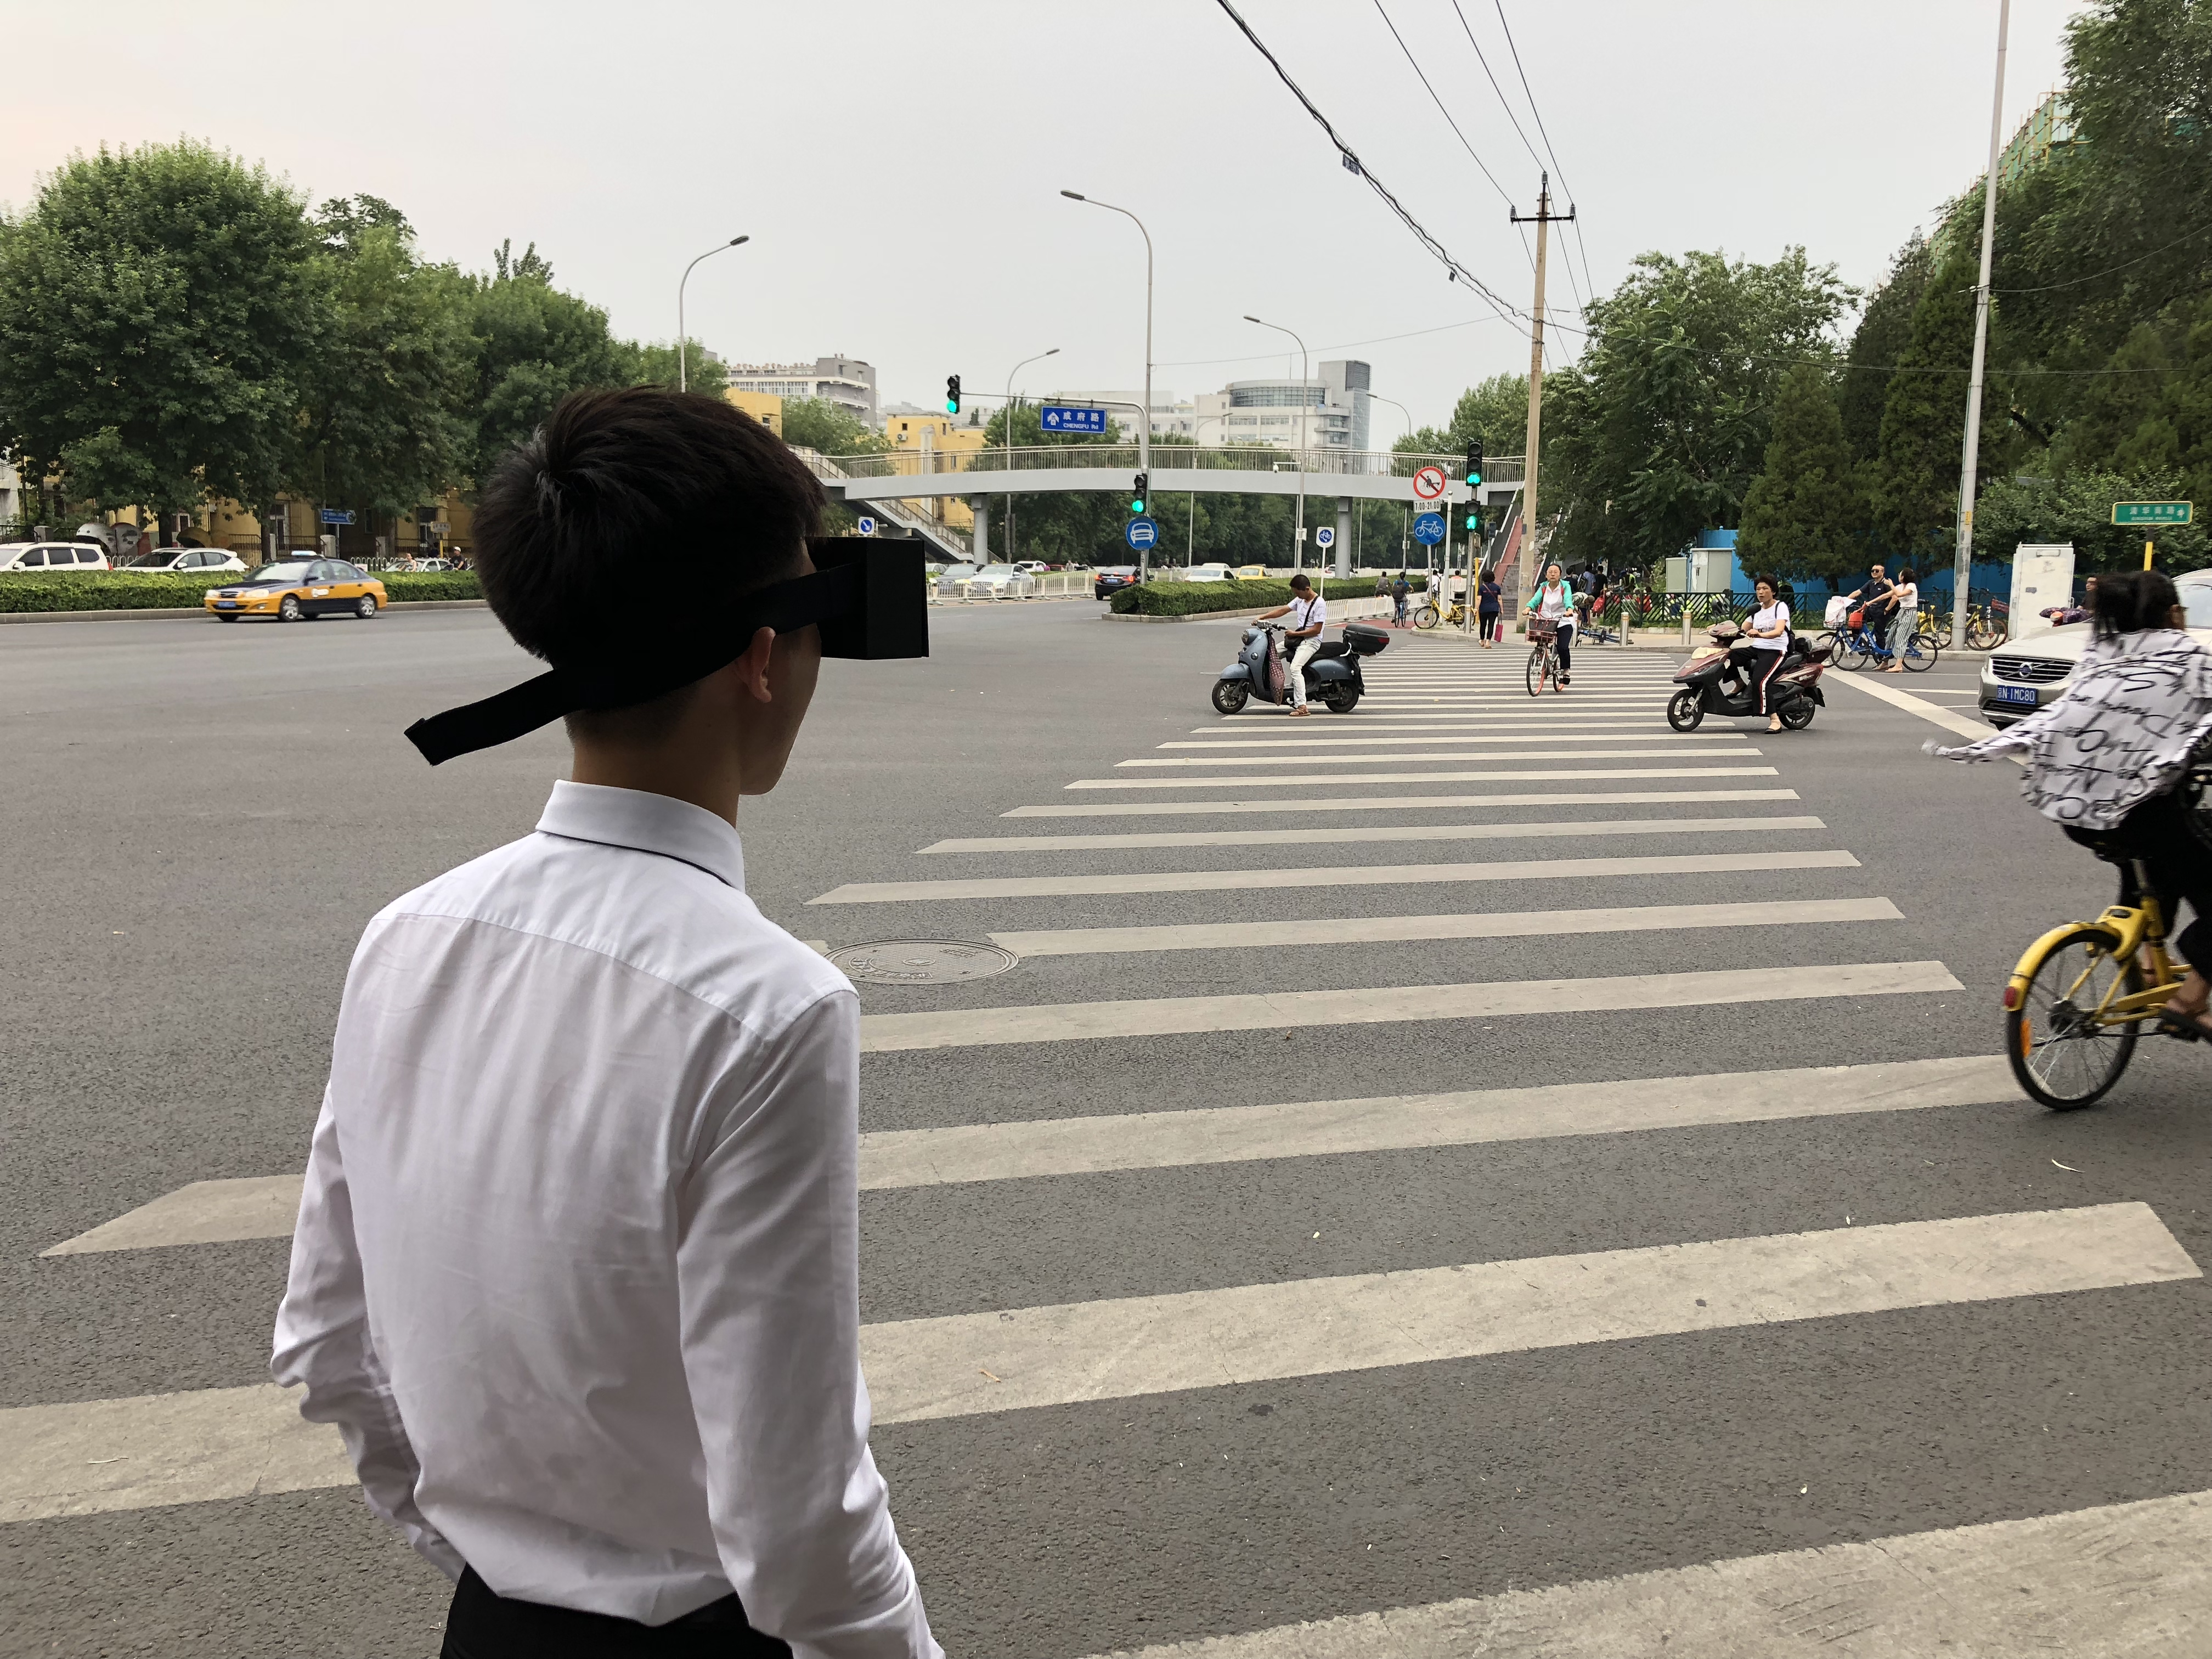
\includegraphics[width=1.\linewidth]{figure/experiment_setting.jpg}
	\end{center}
	\caption{Experiment setting: the user is wearing a RGB camera.}
	\label{fig:expset}
\end{figure}


\para{Results.}
To evaluate the performance of the system, we select a series of representative scenarios from urban road scenes. The properties of the benchmark videos are shown in Table \ref{Table:Benchmarks}. Precision and recall are used as key indicators of the results. The results are shown in Table.  


\begin{table}[!t]
	\centering
	\caption{\footnotesize Properties of the Benchmark Videos}
	\label{Table:Benchmarks}
	%\begin{tabular}{c|c|c}
	 \begin{tabular}{p{1cm}p{4.5cm}p{2cm}}	
		\hline
		Scenario &    Description      &  Total Frames         \\ \hline \hline
		1        &    The red light turns green or the green light turns red. The lights are visible throughout the journey. There is only one pedestrian light in the scene.      &      189    \\ \hline  %video1
		2        & There are multiple traffic lights in the scene. The non-pedestrian lights change their colos (e.g. red to green or green to red). &      162       \\ \hline  %video4
	    3     	 & The zebra crossing is occluded in the distance and the pedestrian light exists in the scene.     &      133       \\ \hline   %video7
		4        & Zebra crossing is in the shade.  &     300      \\ \hline   %video9
		5        & Obstacle avoidance test: pedestrians walk nearby in the same direction. &    258        \\ \hline %video10
		6        & Obstacle avoidance test: pedestrians walk nearby in the opposite direction.   &       271      \\ \hline  %video11
		7        & Obstacle avoidance test: The vehicle is moving laterally in front.   &      340       \\ \hline  %video12
		8        & Pedestrians walk across the road and the pedestrian light stays green for the whole journey.   &       585      \\ \hline  %video15
		9        & Pedestrians walk across the road and the pedestrian light doesn't stay green for the whole journey.   &        158     \\ \hline  %video16
	\end{tabular}
\end{table}









\begin{table}[!t]
	\centering
	\caption{\footnotesize Evaluation Results}
	\label{Table:Results}
	\renewcommand{\multirowsetup}{\centering}
	\begin{tabular}{c|c|c|c|c}
	%\begin{tabular}{p{1cm}p{4.5cm}p{2cm}}	
		\hline
		\multirow{2}[0]{*}{Scenario}  &   \multicolumn{2}{c|}{Detection}    &    \multicolumn{2}{c}{Detection+Tracking}      \\ \cline{2-5}
		 &    Precision      &  Recall   &  Precision & Recall     \\ \hline \hline
		1        &  &    & &            \\ \hline  %video1
		2        &  &    & &            \\ \hline  %video4
		3     	 &  &    & &           \\ \hline  %video7
		4        &  &    & &           \\ \hline  %video9
		5        &  &    & &           \\ \hline  %video10
		6        &  &    & &           \\ \hline  %video11
		7        &  &    & &          \\ \hline  %video12
		8        &  &    & &          \\ \hline  %video15
		9        &  &    & &          \\ \hline  %video16
	\end{tabular}
\end{table}
\include{data/conclusion}


%\section{Related Work}





\section{Acknowledgments}



% Balancing columns in a ref list is a bit of a pain because you
% either use a hack like flushend or balance, or manually insert
% a column break.  http://www.tex.ac.uk/cgi-bin/texfaq2html?label=balance
% multicols doesn't work because we're already in two-column mode,
% and flushend isn't awesome, so I choose balance.  See this
% for more info: http://cs.brown.edu/system/software/latex/doc/balance.pdf
%
% Note that in a perfect world balance wants to be in the first
% column of the last page.
%
% If balance doesn't work for you, you can remove that and
% hard-code a column break into the bbl file right before you
% submit:
%
% http://stackoverflow.com/questions/2149854/how-to-manually-equalize-columns-
% in-an-ieee-paper-if-using-bibtex
%
% Or, just remove \balance and give up on balancing the last page.
%

% REFERENCES FORMAT
% References must be the same font size as other body text.
\bibliographystyle{SIGCHI-Reference-Format}
\bibliography{sample}

\end{document}

%%% Local Variables:
%%% mode: latex
%%% TeX-master: t
%%% End:
